\begin{frame}{Wrinkling of a confined porous layer}

\bigskip
\structure{Fluorescent yoghurt makers}

\bigskip
\begin{tabu}{X[c]X[c]c}
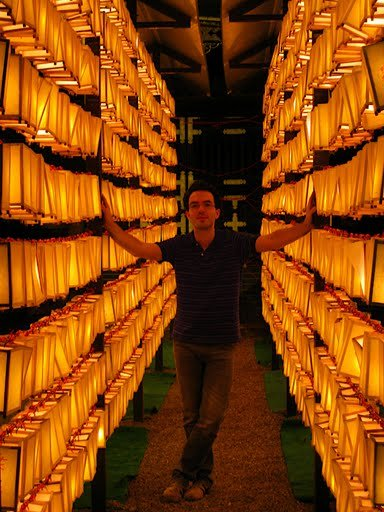
\includegraphics[height=0.3\textheight,clip=true,trim=3cm 7cm  2cm 5cm]{Mathieu}&
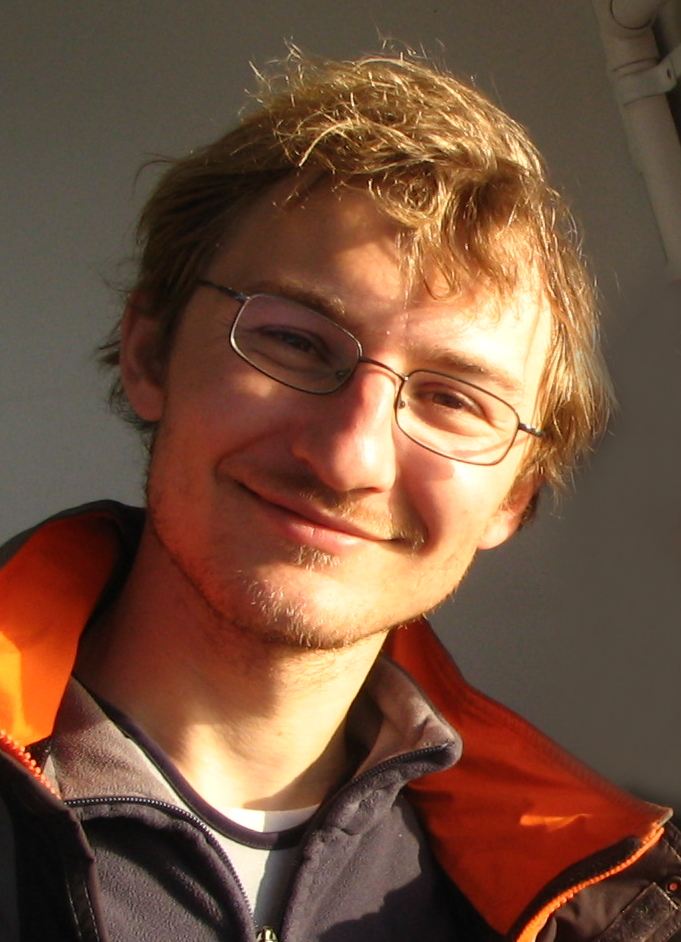
\includegraphics[height=0.3\textheight]{Thomas}&
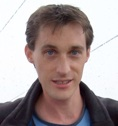
\includegraphics[height=0.3\textheight]{Seb}\\
Mathieu Nespoulous & Thomas Gibaud & Sebastien Manneville\\
Associate Professor & CNRS researcher & Professor\\
Aix-Marseille Université & E.N.S. Lyon & E.N.S. Lyon\\
\end{tabu}

\bigskip
\structure{Imaging plateform} BioSciences Gerland - Lyon Sud (UMS~3444)
\end{frame}

%\tikzset{external/force remake}
\begin{frame}{Over-acidification: Faster but weaker}
\begin{tikzpicture}
\begin{axis}[
	height=0.8\textheight,
	width=\textwidth,
	xlabel={time (h)}, ylabel={$G^\prime$ (\si{\pascal})},
	cycle list name=earthy,
	no marks,
	xmin=0, xmax=20,ymin=0,
	]
	\addplot table[x expr={\thisrowno{0}/3600}]{cas4_GDL1_Y265.prise} node[anchor=base west] {1\%};
	\addplot table[x expr={\thisrowno{0}/3600}]{cas4_GDL1.25_Y277.prise} node[anchor=base west] {1.25\%};
	\addplot table[x expr={\thisrowno{0}/3600}]{cas4_GDL1.5_Y275.prise} node[anchor=base west] {1.5\%};
	\addplot table[x expr={\thisrowno{0}/3600}]{cas4_GDL2_Y268.prise} node[anchor=base west] {2\%};
	\addplot table[x expr={\thisrowno{0}/3600}]{cas4_GDL3_Y270.prise} node[anchor=base west] {3\%};
	\addplot table[x expr={\thisrowno{0}/3600}]{cas4_GDL4_Y271.prise} node[anchor=base west, yshift=-0.2em] {4\%};
\end{axis}
\end{tikzpicture}

Caseins regain some solubility at low pH.
\end{frame}


\begin{frame}{Sealed cell, spontaneous pattern}
	
	\structure{Side view of the cell}\\
	\tikzsetnextfilename{cell_brushes}
	\begin{tikzpicture}[font=\footnotesize]
		\fill[pattern=north east lines,pattern color=Accent2] (0,0) rectangle (\textwidth,1.5em) node[midway,fill=white,inner sep=1pt] {glass};
		\fill[pattern=north east lines,pattern color=Accent2] (0,-2.5em) rectangle (\textwidth,-4em) node[midway,fill=white,inner sep=1pt] {glass};
		\draw[line width=2pt,Accent1] (0.05\textwidth,-2.5em) -- (0.95\textwidth,-2.5em) (0.05\textwidth,-1pt) -- (0.95\textwidth,-1pt) node[below,pos=0.30, text width=0.5\textwidth] {acrylamide brush ($10\sim 100$ nm)\linebreak $\Rightarrow$ No adhesion};
		\fill[gray] (0,0) rectangle (0.05\textwidth,-2.5em) (\textwidth,0) rectangle (0.95\textwidth,-2.5em) node[pos=1, above left] {spacer};
		\draw[<->] (0.75\textwidth,-2pt) -- (0.75\textwidth,-2.5em) node[midway,left] {$e\sim 100\,\mu m$};
		\draw[<->] (0.05\textwidth,2.25em) -- (0.95\textwidth,2.25em) node[midway,above] (L){$L\sim 2.5\,cm$};
		%\node[anchor=north west, inner sep=0] at ($(L.north) - (0.5\textwidth,0)$) {\structure{Side view of the cell}};
	\end{tikzpicture}
	
	\bigskip
	\structure{Top view of the final pattern}\\
	\begin{tikzpicture}[inner sep=0, very thick]
	\setlength{\mylength}{\columnwidth}
	\node[anchor=north west] (a) {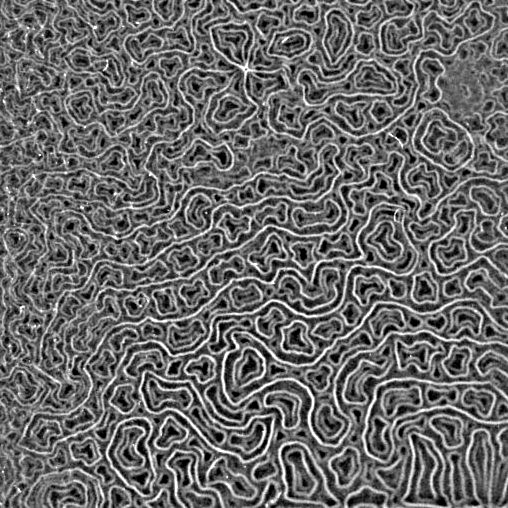
\includegraphics[width=0.28\mylength]{cas3p2_fluo0p8_GDL4_50um_coating_2_zoom2_crop}};
		\node[anchor=north] at (0.44\mylength,0) (b) {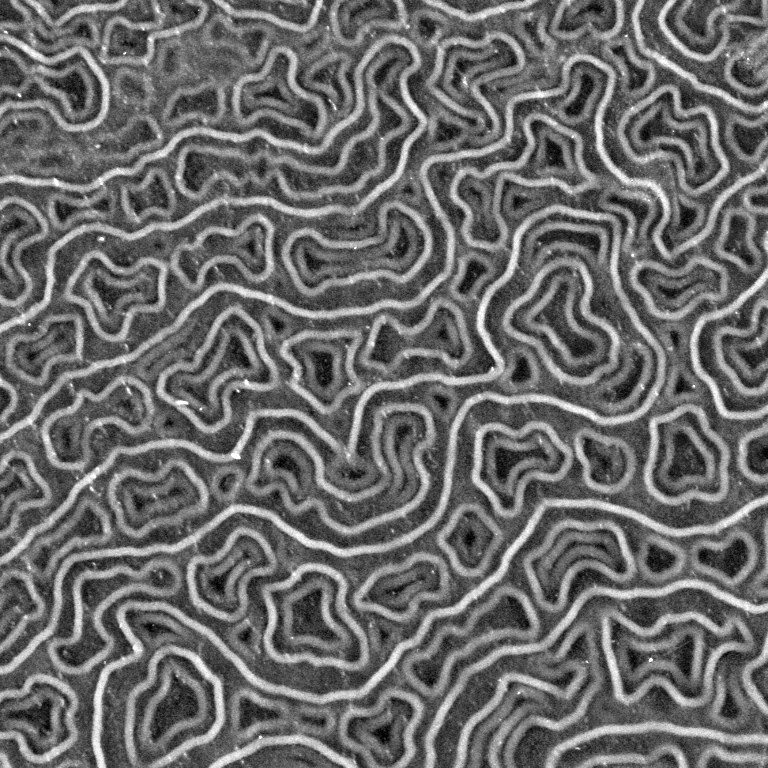
\includegraphics[width=0.28\mylength]{cas3p2_fluo0p8_GDL4_50um_coating_2_zoom6_crop}};
		\node[anchor=north east] at (\mylength,0) (c) {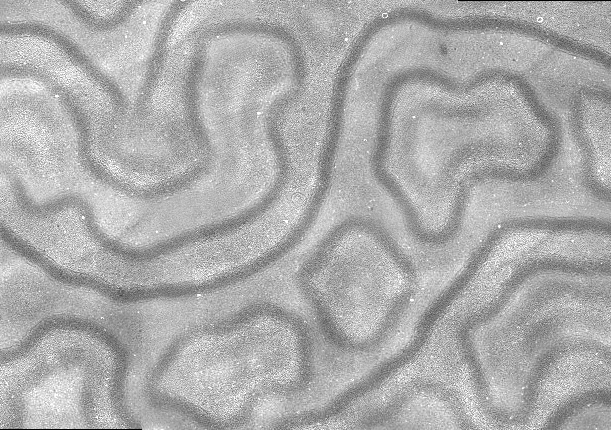
\includegraphics[width=0.4\mylength]{cas3p2_fluo0p8_GDL4_50um_coating_2_transmission}};
		%zooms
		\node[minimum width = 0.137\mylength, minimum height=0.137\mylength, anchor=north west, draw=Accent2] at ($(a.north west) +(0.111\mylength,-0.072\mylength)$) (bz){};
		\draw[Accent2] (bz.north east) -- (b.north west) (bz.south east) -- (b.south west);
		\node[minimum width = 0.128\mylength, minimum height=0.081\mylength, anchor=north west, draw=Main] at ($(b.north west) +(0.097\mylength,-0.143\mylength)$) (cz){};
		\draw[Main] (cz.north east) -- (c.north west) (cz.south east) -- (c.south west);
		\node[minimum width = 0.156\mylength, minimum height=0.156\mylength, anchor=north west, draw=Accent1] at ($(c.north west) + (0.125\mylength,0)$) (dz) {};
		%scale bars
		\draw[ultra thick] (a.south east) ++(0,-0.25em) -- ++(-0.178\mylength,0) node[pos=0.5, below=0.25em, font=\small] (M) {\SI{1}{\centi\metre}};
		\draw[ultra thick] (b.south east) ++(0,-0.25em) -- ++(-0.176\mylength,0) node[pos=0.5, below=0.25em, font=\small] {\SI{5}{\milli\metre}};
		\draw[ultra thick] (c.south east) ++(0,-0.25em) -- ++(-0.132\mylength,0) node[pos=0.5, below=0.25em, font=\small] {\SI{1}{\milli\metre}};
	\end{tikzpicture}
\end{frame}

\begin{frame}{Dynamics (transmission macroscope)}
\movie[externalviewer]{\begin{tikzpicture}
\node[inner sep=0] (a) {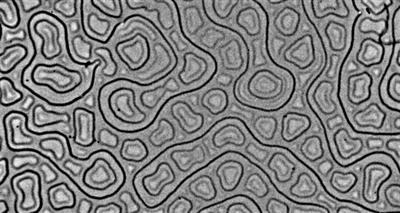
\includegraphics[width=\textwidth]{prise_0799_resized.jpg}};
\draw[line width=0.2em] ++(a.north west) -- ++(0.177\textwidth,0) node[pos=0, above right, inner xsep=0] {\SI{1}{\milli\metre}};
\end{tikzpicture}
}{cas4_GDL_4_100um_coat_macroscope_2.avi}
\end{frame}

\begin{frame}{Dynamics (transmission macroscope)}
\begin{tikzpicture}
	\matrix[matrix of nodes, inner sep=0, column sep=0.015\textwidth, row sep=0.5em, ampersand replacement=\&] (m){
	33 min \& 38 min \& 43 min \\
	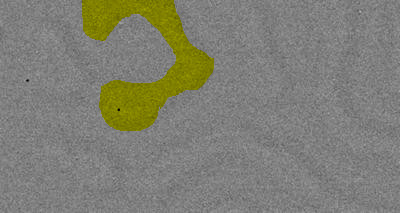
\includegraphics[width=0.32\textwidth]{prise_0100_color.jpg}\&
	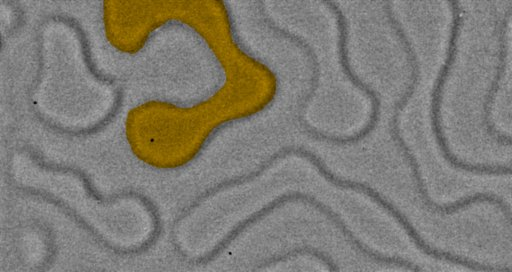
\includegraphics[width=0.32\textwidth]{prise_0130_color.jpg}\&
	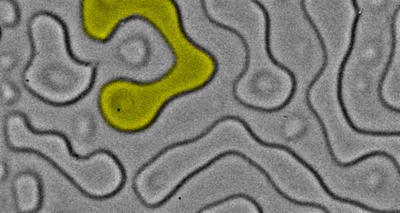
\includegraphics[width=0.32\textwidth]{prise_0160_color.jpg}\\
	48 min \& 1h \& 1h15 \\
	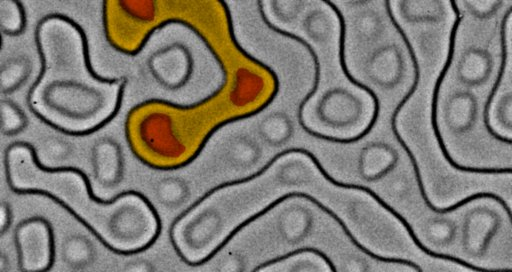
\includegraphics[width=0.32\textwidth]{prise_0190_color.jpg}\&
	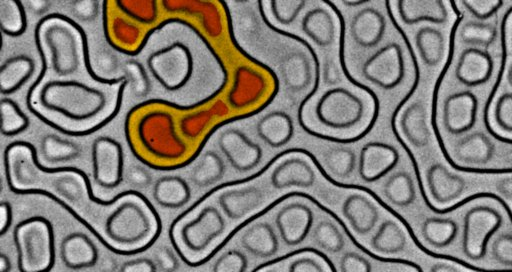
\includegraphics[width=0.32\textwidth]{prise_0250_color.jpg}\&
	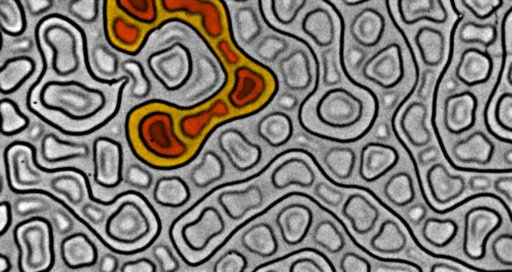
\includegraphics[width=0.32\textwidth]{prise_0360_color.jpg}\\
	};
	\draw[line width=0.2em] ++(m-4-1.south west) -- ++(0.056\textwidth,0) node[pos=0, below right, inner xsep=0] {\SI{1}{\milli\metre}};
\end{tikzpicture}

\begin{itemize}
\item nesting patterns
\item length scale becomes smaller
\end{itemize}
\end{frame}

\begin{frame}{What is going on in the thickness?}
\begin{columns}
\column{0.4\textwidth}
\begin{itemize}
\item fluorescent casein
\item confocal microscope
\item[$\Rightarrow$] 3D concentration field
\end{itemize}

\begin{tikzpicture}
\draw[ultra thick] (0,) -- +(0.786\textwidth,0) node[midway, above] {\SI{1}{\milli\metre}};
\end{tikzpicture}
\setlength{\tabcolsep}{1pt}
\begin{tabular}{p{\columnwidth}l}
	
\includegraphics[width=\columnwidth, height=0.061\columnwidth]{coupe_cloque_t000.png}& \SI{15}{\minute}\\
	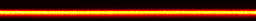
\includegraphics[width=\columnwidth, height=0.061\columnwidth]{coupe_cloque_t011.png} & \SI{22}{\minute}\\
	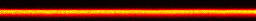
\includegraphics[width=\columnwidth, height=0.061\columnwidth]{coupe_cloque_t110.png} & \SI{1}{\hour}~26\onslide<2->{\\
	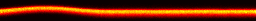
\includegraphics[width=\columnwidth, height=0.061\columnwidth]{coupe_cloque_t116.png} & \SI{1}{\hour}~30\\
	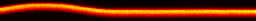
\includegraphics[width=\columnwidth, height=0.061\columnwidth]{coupe_cloque_t117.png} & \SI{1}{\hour}~31\\
	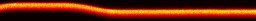
\includegraphics[width=\columnwidth, height=0.061\columnwidth]{coupe_cloque_t123.png} & \SI{1}{\hour}~35\\
	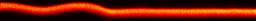
\includegraphics[width=\columnwidth, height=0.061\columnwidth]{coupe_cloque_t200.png} & \SI{2}{\hour}~25\\
	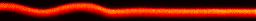
\includegraphics[width=\columnwidth, height=0.061\columnwidth]{coupe_cloque_t221.png} & \SI{2}{\hour}~40\\}
\end{tabular}

\begin{itemize}
\item synæresis and swelling
\item<2-> cause buckling
\end{itemize}
\column{0.1\textwidth}

\column{0.5\textwidth}
\begin{tikzpicture}
	\begin{groupplot}[%
		group style={
			group name=g, group size=1 by 3,
			xticklabels at=edge bottom,
			vertical sep=0,
			},
		xmin=0, xmax=170, xtick={0,30,...,150},
		extra tick style={grid=major},%
		extra x ticks = {21,68}, extra x tick labels={},%
		scale only axis,
		width=\textwidth-4em,
		height=5\baselineskip,
		ylabel absolute, every axis y label/.append style={anchor=base, yshift=-1em}
		]
	\nextgroupplot[
		ylabel={$G^\prime$ (\si{\pascal})},
		ymin=0,
		]
	\addplot+[no marks,Accent1] table[x expr={\thisrowno{0}/60}]{cas4_GDL4_Y271.prise};
	\node[below left] at (rel axis cs:1,1) {rheometer (stick)};
	
	\nextgroupplot[
		ylabel={Volume (\%)}, ymin=20, ymax=100, 
		ytick={40,60,80,100}, every axis y label/.append style={xshift=0.5em},
		]
	\addplot+[no marks,Accent1] table[x expr={\thisrowno{0}+15}, y expr={\thisrowno{1}*100}]{relative_volume_excess_area_cloques.txt};
	%\addplot+[only marks,Accent2, mark=+] table[y expr={\thisrowno{1}*100}]{volume_rel_half_cas8_toi.txt};
	\node[anchor=south west] at (rel axis cs:0,0) {\rotatebox{90}{synæresis}};
	\node at (axis cs:68,80) {swelling};
	
	\nextgroupplot[
		ylabel={Excess area (\%)}, ymin=0, ymax=4, ytick={0,1,2,3},
		xlabel={time (min)}, 
		every axis y label/.append style={xshift=-1em},
		]
	\only<2->{\addplot+[no marks,Accent1] table[x expr={\thisrowno{0}+15}, y expr={\thisrowno{2}*100}]{relative_volume_excess_area_cloques.txt} node[pos=1, below left] {all};
	\addplot+[no marks,Accent2] table[x expr={\thisrowno{0}+15}, y expr={\thisrowno{3}*100}]{relative_volume_excess_area_cloques.txt} node[pos=1, left] {single blister};
	\draw[->] (axis cs: 21, 3) -- (axis cs: 68, 3) node[midway, below] {\SI{1}{\hour}};}
	%\legend{all, single blister};
	\end{groupplot}
	\end{tikzpicture}
\end{columns}
\end{frame}

\begin{frame}{Dynamics (confocal microscope)}
\movie[externalviewer]{\begin{tikzpicture}
	\node[inner sep=0] (a) {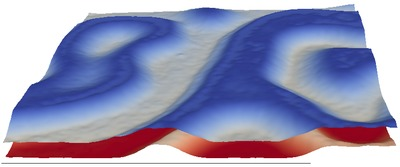
\includegraphics[width=\textwidth]{cas3p2_fluo0p8_GDL4_2_t260_crop_resized.jpg}};
	\draw[line width=0.2em] ++(a.south west) -- ++(0.75\textwidth,0) node[pos=0, below right, inner xsep=0] {\SI{1}{\milli\metre}};
	
	\node[above=1em of a, inner sep=0] (c) {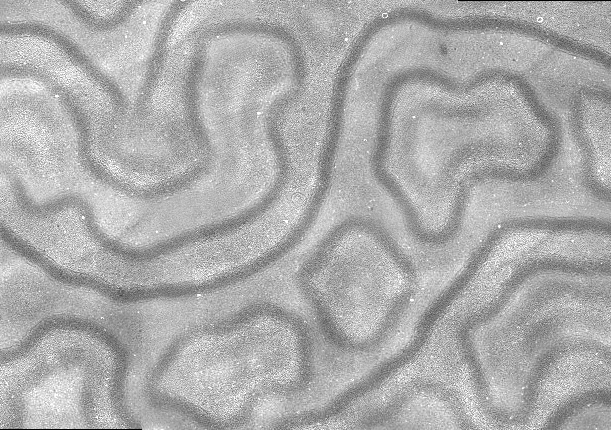
\includegraphics[width=0.4\textwidth]{cas3p2_fluo0p8_GDL4_50um_coating_2_transmission}};

	\node[minimum width = 0.156\textwidth, minimum height=0.156\textwidth, anchor=north west, draw=Accent1] at ($(c.north west) + (0.125\textwidth,0)$) (dz) {};
	\draw[ultra thick] (c.south east) ++(0,-0.25em) -- ++(-0.132\textwidth,0) node[pos=0.5, below=0.25em, font=\small] {\SI{1}{\milli\metre}};
\end{tikzpicture}
}{volume_plis.avi}
\end{frame}

\begin{frame}{Dynamics (confocal microscope)}
\begin{tikzpicture}
	\matrix[matrix of nodes, inner sep=0, column sep=0.015\textwidth, row sep=0.5em, ampersand replacement=\&] (m){
	33 min \& 38 min \& 43 min \\
	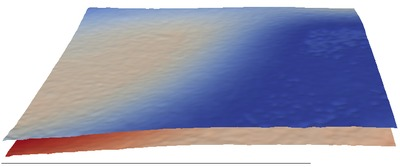
\includegraphics[width=0.32\textwidth]{cas3p2_fluo0p8_GDL4_2_t047_crop_resized.jpg}\&
	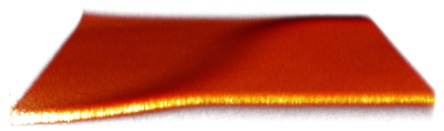
\includegraphics[width=0.32\textwidth]{cas3p2_fluo0p8_GDL4_2_t056_crop_resized.jpg}\&
	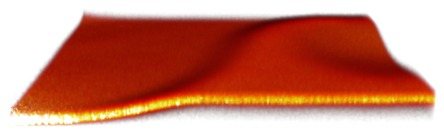
\includegraphics[width=0.32\textwidth]{cas3p2_fluo0p8_GDL4_2_t065_crop_resized.jpg}\\
	48 min \& 1h \& 1h15 \\
	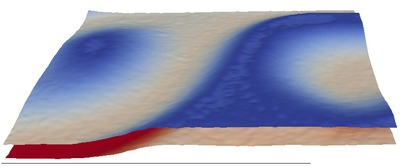
\includegraphics[width=0.32\textwidth]{cas3p2_fluo0p8_GDL4_2_t074_crop_resized.jpg}\&
	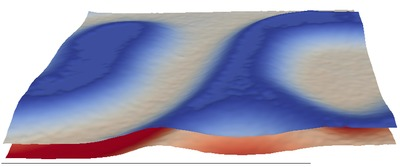
\includegraphics[width=0.32\textwidth]{cas3p2_fluo0p8_GDL4_2_t092_crop_resized.jpg}\&
	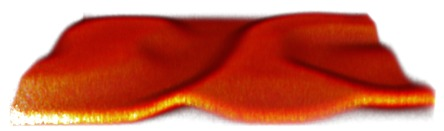
\includegraphics[width=0.32\textwidth]{cas3p2_fluo0p8_GDL4_2_t125_crop_resized.jpg}\\
	};
	\draw[line width=0.2em] ++(m-4-1.south west) -- ++(0.24\textwidth,0) node[pos=0, below right, inner xsep=0] {\SI{1}{\milli\metre}};
\end{tikzpicture}

\begin{columns}
\column{0.32\textwidth}
\begin{itemize}
\item confinement
\item cascade buckling
\item wavelength division
\end{itemize}
\column{0.68\textwidth}
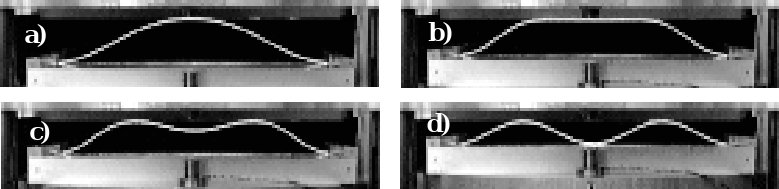
\includegraphics[width=\columnwidth]{Roman_1999_confined.jpg}

\textit{\footnotesize Roman \& Pocheau, EPL (1999)}
\end{columns}

\begin{center}
\alert{Where does the initial wavelength come from?}
\end{center}
\end{frame}


\begin{frame}<1-2>[label=carpet]{Wavelength: resisting stress needed}
\structure{Simple case} Initial flat contact with the substrate: carpet
\begin{columns}
\column{0.5\textwidth}
\temporal<2>{
	
\includegraphics[width=\columnwidth, height=0.061\columnwidth]{coupe_cloque_t000.png}\\
	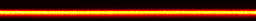
\includegraphics[width=\columnwidth, height=0.061\columnwidth]{coupe_cloque_t011.png}\\
	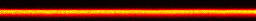
\includegraphics[width=\columnwidth, height=0.061\columnwidth]{coupe_cloque_t110.png}\\
	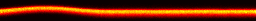
\includegraphics[width=\columnwidth, height=0.061\columnwidth]{coupe_cloque_t116.png}\\
	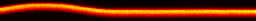
\includegraphics[width=\columnwidth, height=0.061\columnwidth]{coupe_cloque_t117.png}\\

	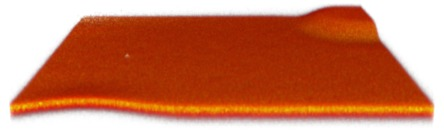
\includegraphics[width=\textwidth]{volume_cloque_t116}\\
	\begin{tikzpicture}
	\draw[ultra thick] (0,) -- +(0.786\textwidth,0) node[midway, below] {\SI{1}{\milli\metre}};
	\end{tikzpicture}
	
	\structure{In our case}
	\begin{itemize}
	\item Vertical cells show the same wavelength
	\item $\sigma \neq \rho g h$
	\end{itemize}
}{

\bigskip
\begin{itemize}
\item solvent must flow through gel
\begin{description}[$\ell_p$]
\item[$v$] gel velocity = -volumic flux $\simeq \SI{0.2}{\micro\metre\per\second}$
\item[$\ell_p$] pore size $ \approx \SI{4}{\micro\metre}$
\end{description}
\item $\sigma$ is a Darcy pressure
\[\sigma = \Delta P \sim \eta h v/\ell_p^2\]
\item poroelastic length
\[ \lambda^* \sim \left(\frac{B \ell_p^2}{\eta v h}\right)^\frac{1}{3} \simeq \SI{2}{\milli\metre}\]
\end{itemize}
}{
\begin{tikzpicture}
\begin{axis}[
	width=\textwidth,
	height=0.6\textwidth,
	xmin=0, xmax=1000, xtick={0,250, 500, 750}, xlabel={position (\si{\micro\metre})},
	ymin=0, ymax=50, ylabel={altitude (\si{\micro\metre})},
	cycle list name=earthy,
	no marks,
	]
	\draw[ultra thick, Accent2] (axis cs:580,0) -- (axis cs:580,50);
	\foreach \x in {2,3,..., 8}
		\addplot table[y index=\x]{alts_bottom_cloque.txt};
\end{axis}
\end{tikzpicture}
\begin{itemize}
\item $\lambda$ frozen at ceiling touch 
\item $A=H\equiv e-h$
\item $\lambda \sim \epsilon^{-3/7} H \sim e$
	%\[ \epsilon \sim \left(\frac{\lambda}{e}\frac{e}{H}\right)^{-7/3} \simeq 0.6\% \]
\end{itemize}
}

\column{0.5\textwidth}
\begin{block}{Ruck in a rug}
\tikzsetnextfilename{ruck}%
\begin{tikzpicture}[ultra thick]
\begin{axis}[
	name=a,
	width=\textwidth, height=3\baselineskip, scale only axis,
	domain=-180:180, no markers, ymin=0, ymax=3,xmin=-180,xmax=180,
	axis lines=none, xtick=\empty,
	axis background/.style={fill=white},
	]
	\addplot+[Accent1]{cos(x)+1};
	\addplot+[Accent1]{cos(x)+1.5};
	\draw[->, Accent2, ultra thick] (axis cs:90,1.25) -- (axis cs:90,2.25) node[pos=1, right] {$v$};
	\draw[Main, ultra thick, {Circle}->] (axis cs:-90,1.5) -- (axis cs:-90,0.25) node[right] {$\sigma$};
	%\node[above] at (axis cs:-90,1.5) {$P_2$};
	%\node[below right] at (axis cs:-90,1.25) {$P_1$};
	\draw[<->, ultra thick] (axis cs:0,0) -- (axis cs:0,2) node[midway, right] {$A$};
	\draw[<->] (axis cs:0,2) -- (axis cs:0,2.5) node[midway, right] {$h$};
\end{axis}
\fill[pattern=north east lines,pattern color=Accent2] (a.south west) rectangle ($(a.south east)+(0,-1em)$);
\draw[<->] ($(a.south west)+(0,-1.1em)$) -- ($(a.south east)+(0,-1.1em)$) node[midway, below] {$\lambda$};
\end{tikzpicture}

\textit{\footnotesize Kolinski et al., Vella et al. PRL 2009}\\
\begin{description}[$B$]
\item[$\epsilon$] excess area \hfill$\Rightarrow$ buckling 
\item[$B$] bending modulus \hfill$\Rightarrow \lambda\nearrow$
\item[$\sigma$] vertical stress \hfill$\Rightarrow \lambda\searrow$
\end{description}
\[ \lambda^* \equiv \left(\frac{B}{\sigma}\right)^{1/3}\text{, eg. }\sigma =\rho g h \]
$\lambda \sim \epsilon^{1/7} \lambda^*$ and $A \sim \epsilon^{4/7} \lambda^*$
\end{block}
\end{columns}
\end{frame}

\begin{frame}{Poroelasticity}
\begin{columns}\column{0.15\textwidth}
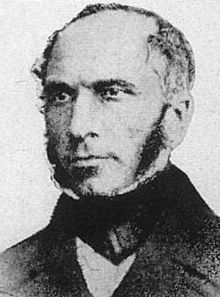
\includegraphics[width=\textwidth]{Henry_Darcy}
\column{0.85\textwidth}
\begin{block}{Henry Darcy (1803-1858)}
\begin{description}[1803]
\item[1846] granted lifelong free water
\item[1856] \textit{Les fontaines publiques de la ville de Dijon}
\end{description}
\end{block}
\end{columns}

\begin{columns}
\column{0.15\textwidth}
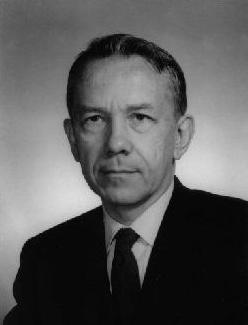
\includegraphics[width=\textwidth]{Maurice_Anthony_Biot}
\column{0.58\textwidth}
\begin{block}{Maurice Anthony Biot (1905-1985)}
\begin{description}[1803]
%\item[1932] Ph.D. under von Kármán (Cal Tech)
\item[1932-1942] earthquake engineering
\item[1935-1962] theory of poroelasticity
\end{description}
\end{block}
\column{0.27\textwidth}
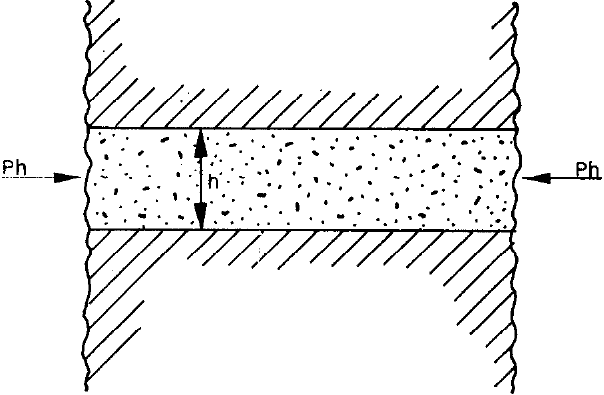
\includegraphics[width=\textwidth]{Biot_1964_Buckling_Porous}
\end{columns}

\medskip
\begin{footnotesize}
\textit{Biot, J. Appl. Mech. 1964}: Buckling of a porous slab embedded in an impervious infinite viscous or viscoelastic medium
\end{footnotesize}
\begin{itemize}
\item $B$ transiently higher due to pore pressure
\item $\sigma$ comes only from the surrounding medium $\rightarrow 0$
\item effect of flow through the porous slab not considered
\end{itemize}
\end{frame}

\begin{frame}{No initial contact with a substrate}
\structure{Poiseuille vs Darcy on a flying carpet}
\begin{tikzpicture}
\begin{axis}[
	name=a,
	width=\textwidth, height=0.25\textwidth, scale only axis,
	domain=0:360, no markers, ymin=-4, ymax=4,xmin=0,xmax=360,
	axis lines=none, xtick=\empty,
	]
	\fill[gray!20] (axis cs:85,4) rectangle (axis cs:95,-4) (axis cs:265,4) rectangle (axis cs:275,-4);
	\addplot+[Accent1]{sin(x)+0.5};
	\addplot+[Accent1]{sin(x)-0.5};
	\addplot+[dashed, black]{0.5};
	\addplot+[dashed, black]{-0.5};
	\draw[<->, help lines] (axis cs:180,0.5) -- (axis cs:180,4) node[midway, left] {$H$}; 
	\draw[<->, help lines] (axis cs:30,-0.5) -- (axis cs:30,-4) node[midway, left] {$H$};
	\node[below] at (axis cs:90,-1.5) (pb1) {$P_1$};
	\node[above] at (axis cs:90,1.5) (ph2) {$P_2$};
	\node[above] at (axis cs:270,1.5) (ph1) {$P_1$};
	\node[below] at (axis cs:270,-1.5) (pb2) {$P_2$};
	\draw[line width=0.1em, ->] (ph2) -- (axis cs:90,0.5) node[midway, left] {Darcy} node[midway, right] {$v$};
	\draw[line width=0.1em, ->] (pb2) -- (pb1) node[midway, above] {Poiseuille} node[midway, below] {$u \sim \frac{\lambda}{H} v$};
\end{axis}
\fill[pattern=north east lines,pattern color=Accent2] (a.south west) rectangle +(\textwidth,-1em) (a.north west) rectangle +(\textwidth,1em);
\end{tikzpicture}

\begin{columns}
\column{0.83\textwidth}
\begin{itemize}
\item The same $\Delta P$ can be relaxed by a Poiseuille flow
\[\Delta P \sim 12\eta\frac{\lambda}{H^2} u \sim 12\eta\frac{\lambda^2}{H^3} v\]
\item For the same wavelength
\hfill$\displaystyle \frac{v_\text{Darcy}}{v_\text{Poiseuille}} \sim \frac{\ell_p^2\lambda^2}{hH^3} \approx 30$
\item Flow through the pores dominates
\end{itemize}
\column{0.17\textwidth}
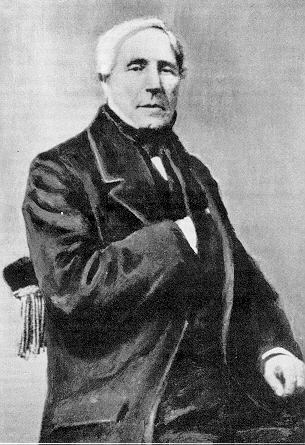
\includegraphics[width=\textwidth]{Jean-Leonard-Marie_Poiseuille.jpg}\\
\hfill\structure{1797-1869}
\end{columns}
\end{frame}

\againframe<3>{carpet}

%\tikzset{external/force remake}
\begin{frame}{Cell thickness}
\begin{tikzpicture}[mark size={0.3em}]
	\matrix[matrix of nodes, inner sep=0, column sep=0.01\columnwidth, row sep=0.01\columnwidth, ampersand replacement=\&] (m) {
		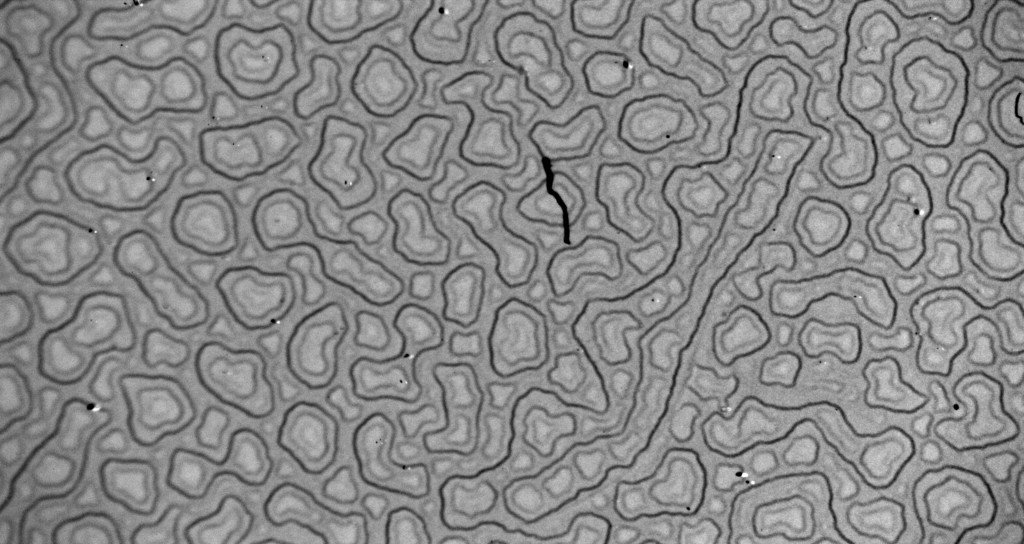
\includegraphics[width=0.245\columnwidth]{pattern_50um.jpg}\&
		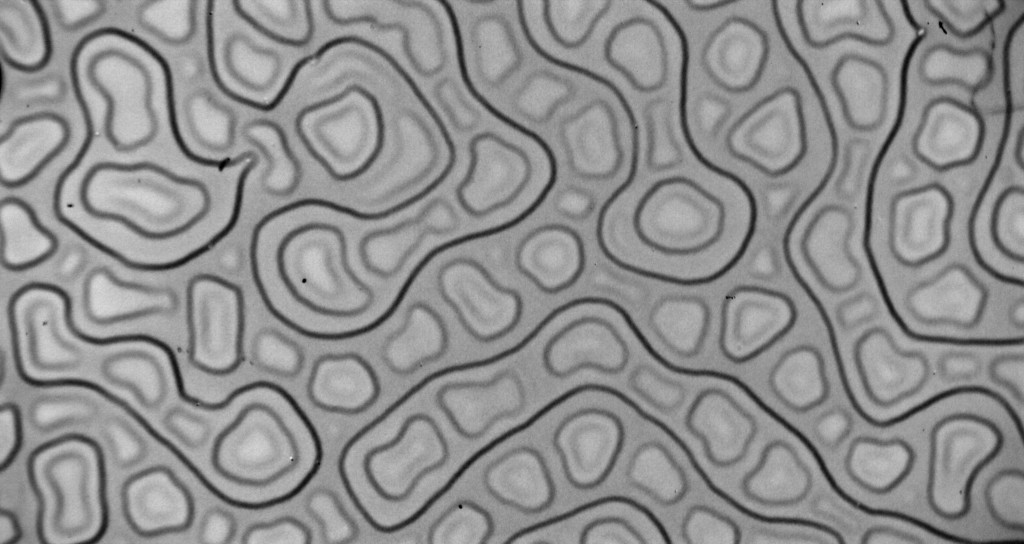
\includegraphics[width=0.245\columnwidth]{pattern_100um.jpg}\&
		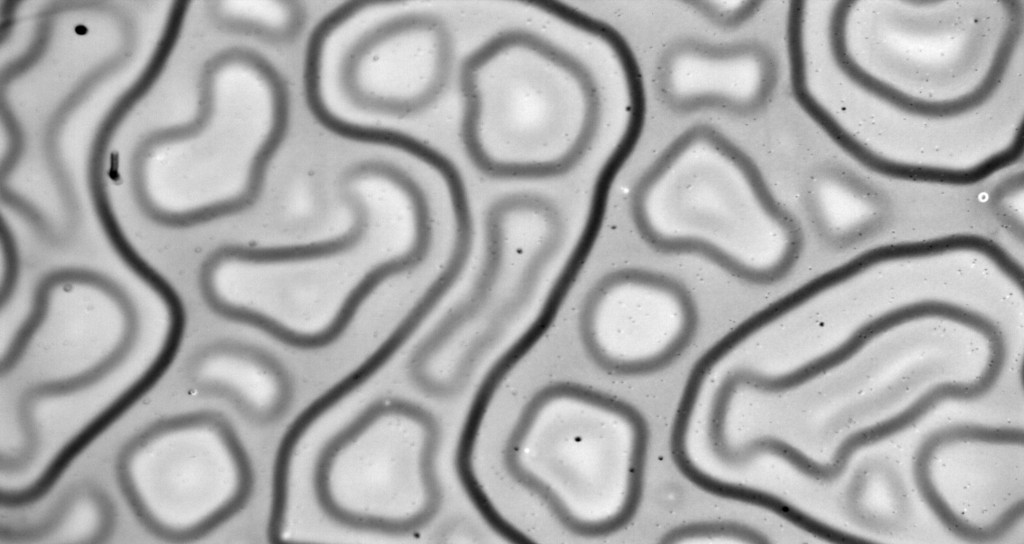
\includegraphics[width=0.245\columnwidth]{pattern_250um.jpg}\&
		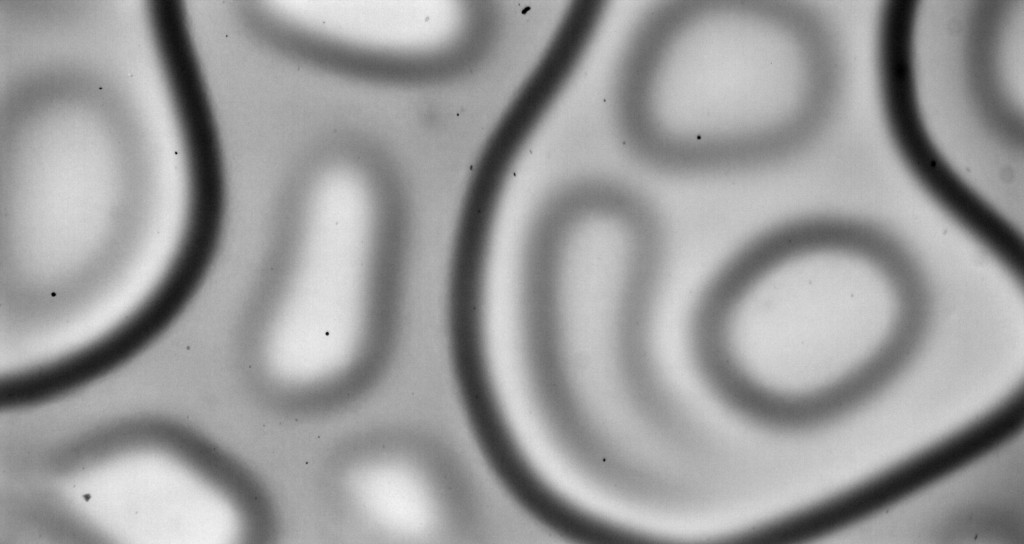
\includegraphics[width=0.245\columnwidth]{pattern_450um.jpg}\\
	};
	\node[inner sep=0, below left=0.01\columnwidth and 0 of m.south east] (x800) {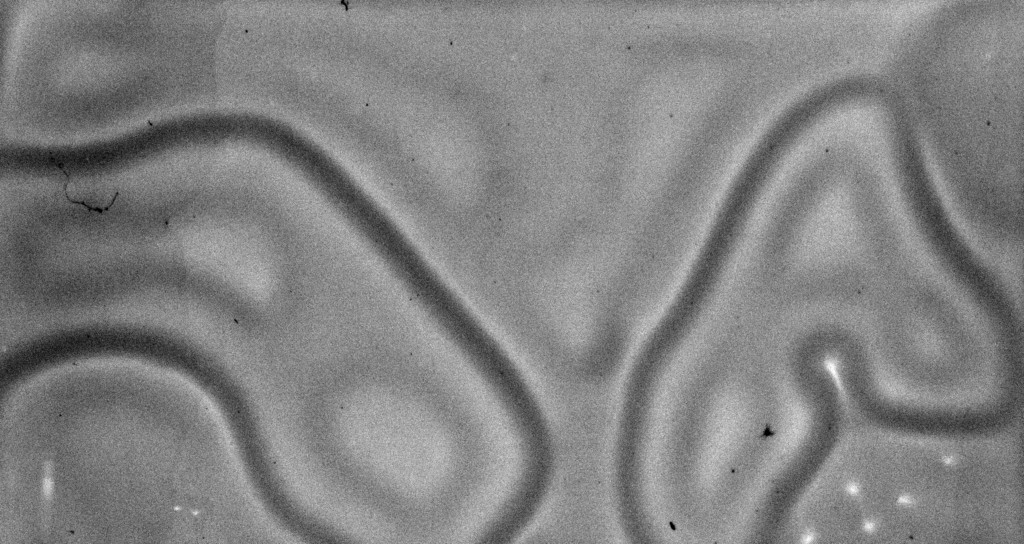
\includegraphics[width=0.49\columnwidth]{pattern_800um_x1.jpg}};
	\draw[ultra thick, Accent2, <->] (x800.south west) ++(0.196\columnwidth, 0.05\columnwidth) -- ++(0.145\columnwidth,0) node[midway,above]{$\lambda$};
	\draw[line width=0.2em,Main](x800.north east) -- ++(-0.217\columnwidth,0) node[midway,below] {\SI{5}{\milli\metre}};
	
	\begin{axis}[%
		name=g,
		anchor=left of north west,
		at={($(m.south west)+(0,-0.01\columnwidth)$)},
		scale only axis,
		width=0.5\textwidth-3em,
		height=0.25\columnwidth-2em,
		xmin=0,xmax=1,xlabel={$e$ (\si{\milli\metre})},
		xtick={0,0.4,...,0.9},
		ymin=0,ylabel={$\lambda$ (\si{\milli\metre})},
		]
		\addplot[no marks, domain=0:3] {4.23*x};
		\begin{scope}[inner sep=0, minimum size=0.8em]
			\node[circle, fill=Accent1] at (axis cs:0.05,0.261){};
			\node[circle, fill=white, draw=Accent1] at (axis cs:0.1,0.458) {};
			\node[regular polygon, regular polygon sides=3, fill=Accent1] at (axis cs:0.250,0.916){};
			\node[regular polygon, regular polygon sides=3, fill=white, draw=Accent1] at (axis cs:0.450,2.075){};
			\node[fill=Accent1] at (axis cs:0.800,3.333){};
		\end{scope}
	\end{axis}
	\begin{scope}[inner sep=0, minimum size=0.8em, transform canvas={xshift=0.5em, yshift=-0.5em}]
		\node[circle, fill=Accent1] at (m-1-1.north west) {};
		\node[circle, fill=white, draw=Accent1] at (m-1-2.north west){};
		\node[regular polygon, regular polygon sides=3, fill=Accent1] at (m-1-3.north west){};
		\node[regular polygon, regular polygon sides=3, fill=white, draw=Accent1] at (m-1-4.north west) {};
		\node[fill=Accent1] at (x800.north west) {};
	\end{scope}
\end{tikzpicture}
\end{frame}
%\tikzset{external/force remake=false}

\tikzset{external/force remake}
\begin{frame}{Surprising viscosity influence}
\begin{columns}
\column{0.5\textwidth}
\[ \lambda^* \sim \left(\frac{B \ell_p^2}{\eta v h}\right)^\frac{1}{3}\]
\begin{tikzpicture}
	\begin{loglogaxis}[%
		width=\textwidth,
		height=0.8\textwidth,
		xmin=0.6,xmax=11,xlabel={viscosity (\si{\milli\pascal\second})},
		xtick={0.7, 1, 2, 5, 10}, xticklabels={$0.7$, $1$, $2$, $5$, $10$},
		ytick={1,2,3,4}, yticklabels={$1$,$2$,$3$,$4$},
		ymin=1, ymax=5, ylabel={$\lambda$ (\si{\milli\metre})},
		mark size={0.3em},
		legend style={legend pos=south east},
		]
		\addplot+[no marks, domain=0.7:10, black, forget plot] {1.7*x^0.4} node[midway, below] {$\eta^{0.4}$};
		\addplot+[only marks,Accent1, mark=o] table{eta_lambda_eau_pure.txt};
		\addplot+[only marks,Accent2, mark=square] table{eta_lambda_eau_glycerol.txt};
		\legend{water, water-glycerol};
	\end{loglogaxis}
\end{tikzpicture}

\column{0.5\textwidth}
\begin{itemize}
\item $\lambda$ increases with $\eta$
\item Can be explained only by a hidden dependence of the viscosity on $B$, $\ell_p$, \ldots 
\item[$\Rightarrow$] Viscosity influences gel formation.
\end{itemize}
%If $\ell_p \sim \eta^{-\alpha}$ and $B\sim \mathrm{k_B}T \left(\frac{h}{\ell}\right)^3$, then
%\[ \lambda^* \sim \eta^\frac{\alpha-1}{3} \]
%\[\alpha\simeq 2.2\]
\end{columns}
\end{frame}

\begin{frame}{Viscosity of the solvent during gel formation}
\begin{tabu}{X[c]X[c]}
water, $\eta=\SI{1}{\milli\pascal\second}$ &
glycerol 60\%, $\eta=\SI{10}{\milli\pascal\second}$\\
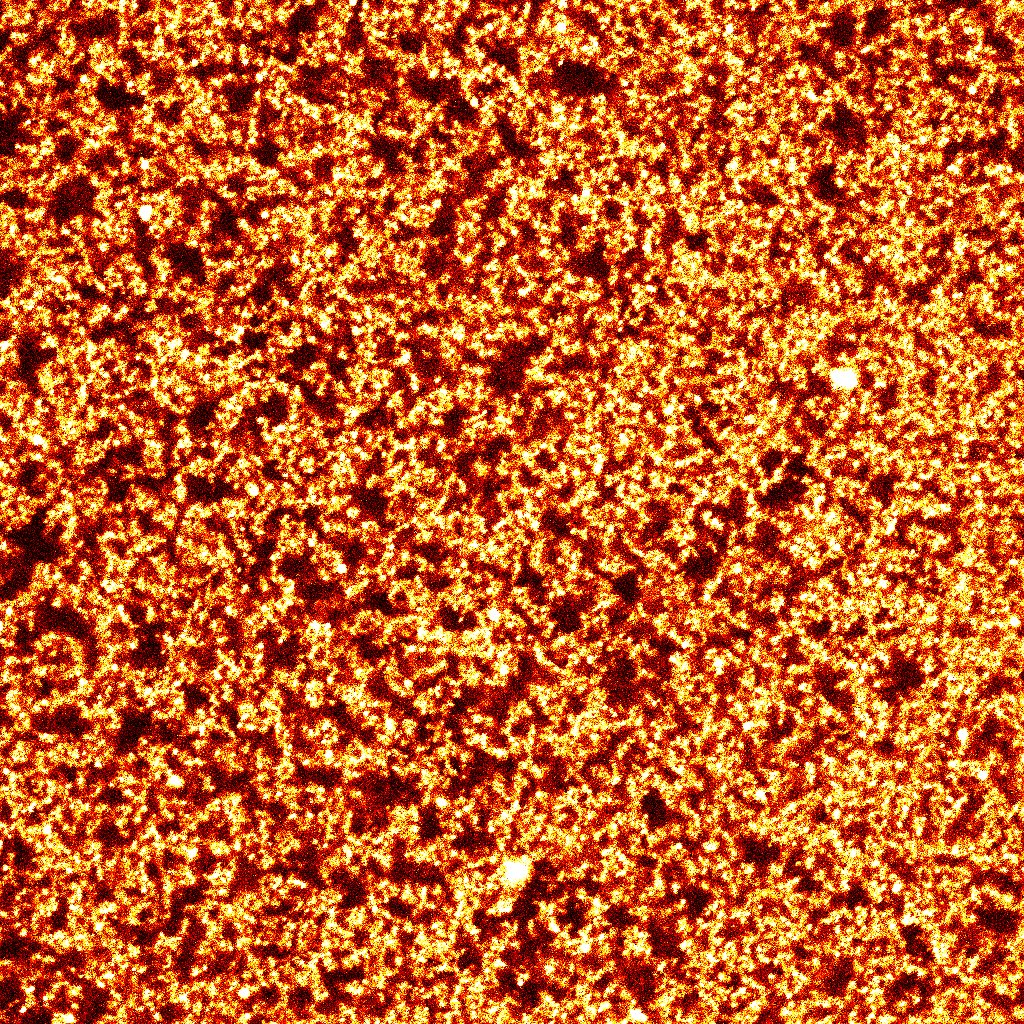
\includegraphics[width=0.45\textwidth]{XYslice_gly0}&
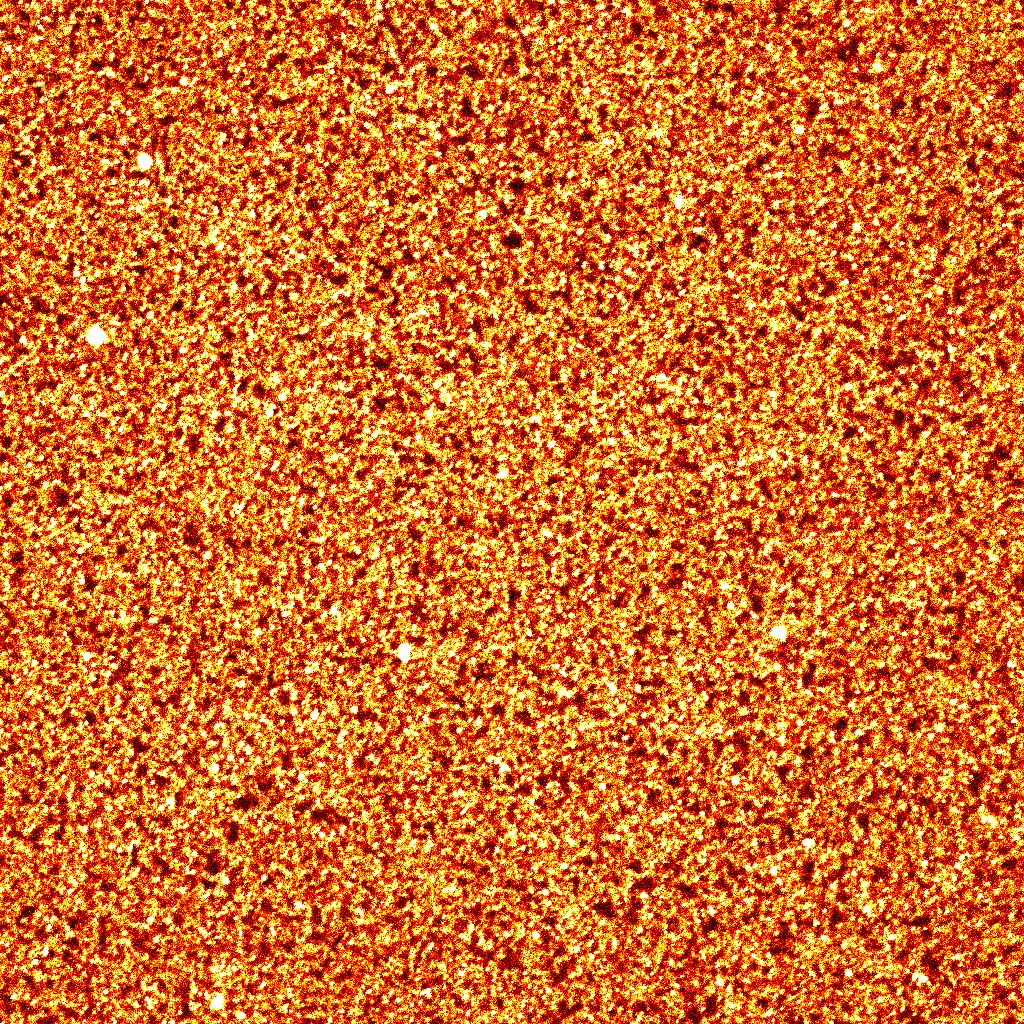
\includegraphics[width=0.45\textwidth]{XYslice_gly60}
\end{tabu}
\tikz\draw[line width=0.2em] (0,0) -- ++(0.045\textwidth,0) node[midway, below] {\SI{10}{\micro\metre}};
\end{frame}

\begin{frame}{Conclusion}
Spontaneous wrinkling of over-acidified casein gels in non-adhesive confinement
	
	\structure{Original patterns}
	\begin{itemize}
		\item nested (optical elements ?)
		\item kinetic wavelength selection
	\end{itemize}
	\structure{A new wrinkling mechanism}
	\begin{itemize}
		\item porous flow resist bending
		\item Darcy can beat Poiseuille
		\item may extend to other porous sheets (wet paper, biological membranes\ldots)
	\end{itemize}
	\structure{Viscosity influences}
	\begin{itemize}
		\item porous dissipation
		\item gel formation (theory?)
		\raisebox{0.6\normalbaselineskip}[0pt][0pt]{$\left.\rule{0pt}{1.1\normalbaselineskip}\right\}$ thus wrinkling}
	\end{itemize}
	\structure{To do:} Measure everything to plot $\lambda_\text{theory}$ vs $\lambda_\text{experiment}$
\end{frame}
